\label{fs-framework}

Let us consider the news topic classification as an illustration of a text stream multi-classification task. There are two input streams: pre-labeled and raw. The latter stream elements must be labeled by a classifier and delivered to end-user. The pre-labeled stream is used for updating a machine learning model with new data. The ultimate purpose is to achieve the distribution of news topics that is changed over time. This task is a typical representative of the text stream classification problem.

As the main requirement to a stream processing engine we claim the following: each output element must depend only on the input. In other words, node failures and execution environment parameters must not affect the results, similar to batch systems. Otherwise, it is hard to design a solution that provides reproducible and interpretable classification results at scale.

The introduced requirement affects the choice of a delivery guarantee. If a stream processing system provides {\em at least once}, some input texts can be processed more than one time in case of failures. This behavior may lead to biased prediction results. For example, if a single sports article is processed many times due to multiple failures, the resulted topics distribution will show that sport is a hot news topic right now. Hence, the only suitable delivery guarantee is {\em exactly once}.

\subsection{Na\"ive data flow}

\begin{figure}[htbp]
  \centering
  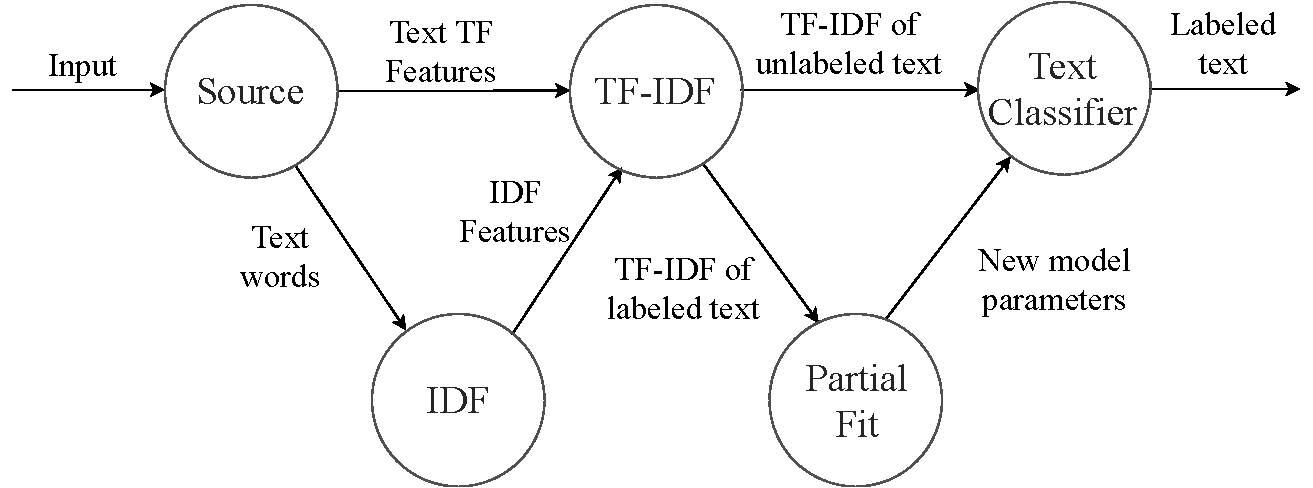
\includegraphics[scale=0.38]{pics/logical-graph}
  \caption{The na\"ive data flow}
  \label {logical_graph}
\end{figure}

Typical classification pipeline based on bag-of-words text representation consists of three steps. The first one is computing TF-IDF features. The second one is training a classifier on these features or making a prediction. For the adaptation of this pipeline for a stream processing engine, there is a need to represent it in the form of a {\em logical graph}. It serves as a descriptive language for defining streaming computations. Vertices of a logical graph denote operations, while edges indicate data subscriptions between them. 

The initial point in our data flow is an {\em Source} vertex. It receives input texts from data producers and computes term frequencies. Computing of inverse document frequencies is a separate operation because it maintains a state and requires different data partitioning in a physical execution that we touch upon further. {\em TF-IDF} vertex joins features corresponding to the same text and passes them to the {\em Text Classifier}. {\em Text Classifier} is the very last vertex that predicts a label and delivers it to a data consumer. The scheme of the proposed logical graph is shown in Figure~\ref{logical_graph}.

Training pipeline is a separate branch within the logical graph introduced above. For already labeled text its features are sent to a {\em Partial fit} vertex instead of the {\em Classifier}. {\em Partial fit} vertex buffers all input elements until training is triggered. After training, the buffer flushes. Updated parameters of a machine learning model are saved for further training and broadcasted to all {\em Text Classifier} vertices.

An issue regarding this pipeline is that the training process may be time-consuming. If training and prediction processes run consequently, there will be significant latency spikes, e.g. if a training process lasts for several minutes, then spikes may be 10 000 times greater than latency for prediction. However, without synchronization, there will be no reproducible correspondence between texts and applied model. It is almost impossible to achieve the same results within a new run on the same data because the training time becomes a hidden parameter that influences output. For instance, assume that we make two runs. On the first run model update consumes 1 minute, but on the second run 2 minutes due to extra CPU load. If training and predicting are not synchronized, more unlabeled input elements are processed by an updated model in the first case, so the distribution of news topics may be completely different between these two runs. 

\begin{figure}[htbp]
  \centering
  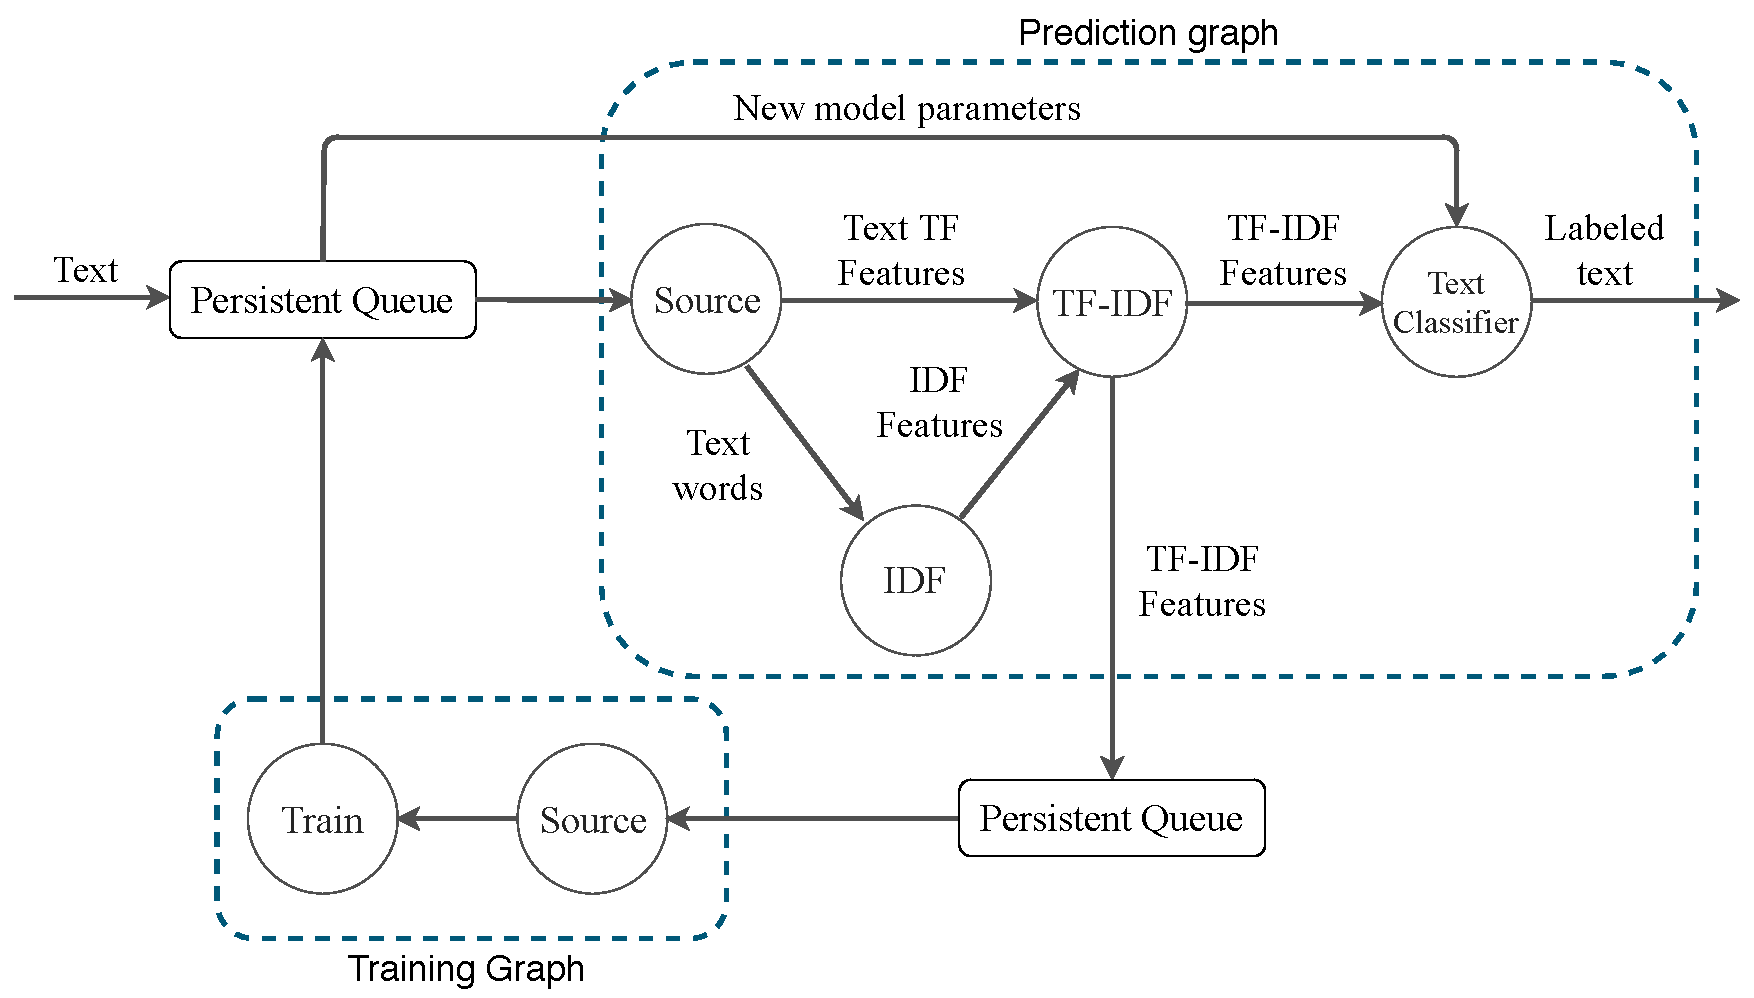
\includegraphics[scale=0.300]{pics/pipeline}
  \caption{The reproducible data flow}
  \label {pipeline}
\end{figure}

\begin{figure}[htbp]
  \centering
  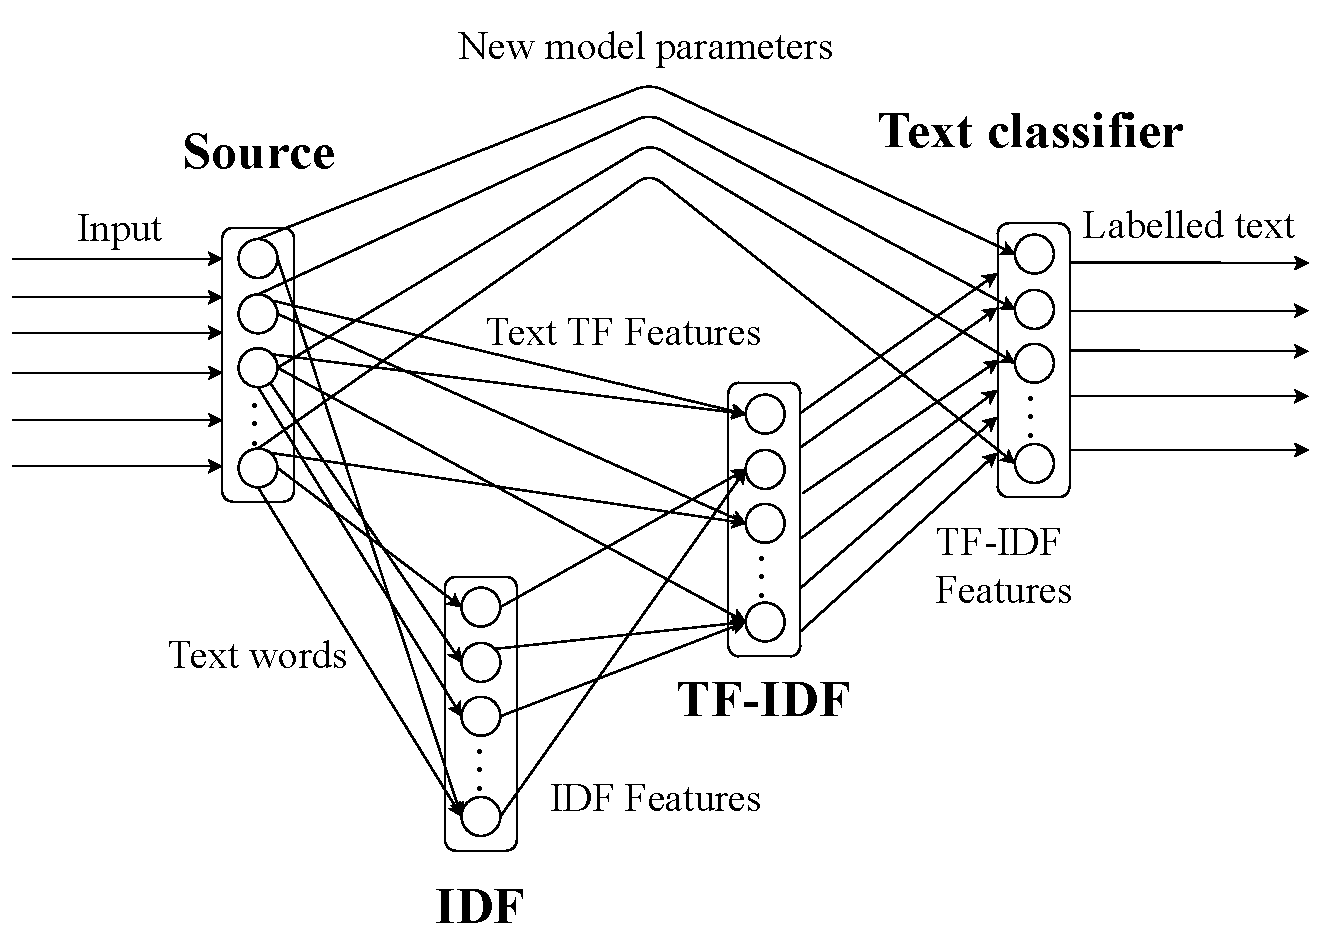
\includegraphics[scale=0.375]{pics/physical-graph}
  \caption{The physical prediction graph}
  \label {physical_graph}
\end{figure}

\subsection{Reproducible data flow}

While the proposed above data flow can fit in requirements for some applications, it is still unsuitable for many production-ready solutions that aim to low latency and reproducibility. We propose two solutions for the mentioned issue:

\begin{itemize}
    \item Use online learning algorithms. In this case, model updating is smooth and its synchronization with training does not cause latency spikes.
    \item Consider model parameters as special input elements that are stored with other input elements in a persistent queue, e.g. Kafka~\cite{kreps2011kafka}. To reproduce results, there is just a need to replay elements from this queue.
\end{itemize}

In this work, we apply the second approach, while the first one is related to our future work. Model parameters are computed as another pipeline in the same streaming system. The scheme is shown in Figure~\ref{pipeline}. This solution also requires enforcing the order in a data flow. Let us demonstrate it by a typical execution of the proposed logical graph that is captured in Figure~\ref{physical_graph}. Each vertex on the scheme denotes the same computational cluster consisted of multiple units. Data partitioning before {\em IDF} and {\em TF-IDF} operations is defined by keys. Data elements with the same keys process on a single computational unit. For {\em IDF} operation the key is a word, while {\em TF-IDF} aggregates items with the same text identifier. 

The issue here is that there can be a race between model updates and computing of {\em TF-IDF}. Even if the correspondence between model parameters and input texts is defined by a persistent queue, they can be reordered during the physical execution. The solution to this problem is specific for a concrete streaming engine.

\subsection{Stream processing systems}

As it was demonstrated above, {\em exactly once} is a strong requirement for the text classification pipeline. On the other hand, the key performance metric in streaming applications is latency, so there is a need to achieve as small latency as possible. Table~\ref{comparison} shows if a system supports exactly once and low latency (less than 500 ms). As we can see, among open systems only~\FlameStream\ provides for both low latency and exactly once. This property is achieved using optimistic order enforcement that implies system-wide idempotence. The details of this approach are discussed in~\cite{we2018adbis, we2018beyondmr}. Further, in experiments, we use~\FlameStream\ engine.

\begin{table}[htbp]
\begin{threeparttable}
\begin{tabular}{lcl}
System             & Exactly-once & Latency    \\
\hline
Storm,Heron,Samza  &    --         &   low            \\
Spark Streaming    &    +          &   high           \\
Flink              &    +          &   high$^*$       \\
MillWheel          &    +          &   NA             \\
FlameStream        &    +          &   low            \\
\end{tabular}
* with enabled exactly-once~\cite{we2018beyondmr}
\end{threeparttable}
\caption{Support of exactly and low latency (less than 500ms) by stream processing systems}
\label{comparison}
\vspace{-6mm}
\end{table}